\documentclass[11pt]{article}
%\documentclass[12pt]{article}

\usepackage[T1]{fontenc}
\usepackage[scaled=1.0]{helvet}
\renewcommand{\familydefault}{\sfdefault}

% margins >=2cm
%\usepackage[a4paper,margin=2cm]{geometry}
\usepackage[a4paper,top=2.1cm,bottom=1.5cm,right=2cm,left=2cm]{geometry}
\footskip 18pt

%\parindent=0.0in
%\parskip=5pt

\usepackage{graphicx, color, tabularx, multirow, setspace, url,titling}
\usepackage{amsmath,bm}
\usepackage{multicol}
\setlength{\columnsep}{0.8cm}
%\usepackage{wrapfig}
%\usepackage[justification=centering]{caption,subfig}
\usepackage[justification=centering]{subfig}
%\renewcommand{\baselinestretch}{1.6}

% Crossing out and new text in different colours for different authors
\usepackage{xparse}
\usepackage{soul,soul}
\usepackage{xcolor}

\newcommand{\HWnew}[1]{#1} %{\color{red}#1}}
\newcommand{\ICnew}[1]{} %{\color{blue}#1}}
\newcommand{\HWcomment}[1]{}%{{\color{red}{#1}}}
\newcommand{\ICcomment}[1]{}% {\it\color{blue}[#1]}}
\newcommand{\HWcrossOut}[1]{}
\newcommand{\ICcrossOut}[1]{}

\usepackage{float}

% make floats take up less space
\setlength{\textfloatsep}{1ex}
\setlength{\abovecaptionskip}{0.1ex}
%% \belowcaptionskip: space below caption

% tabularx stuff
\newcolumntype{Y}{>{\raggedright\arraybackslash}X}
\renewcommand{\tabularxcolumn}[1]{>{\raggedright\arraybackslash}p{#1}}
%\renewcommand{\tabularxcolumn}[1]{>{\raggedright\arraybackslash}m{#1}}

%%% modifications to make article style more compact
\makeatletter

\newenvironment{tablehere}
  {\def\@captype{table}}
  {\vskip 1em}

\newenvironment{figurehere}
  {\def\@captype{figure}}
  {\vskip 1em}

\def\@part[#1]#2
{%
    \refstepcounter{part}%
    {%
        \parindent \z@ \raggedright \interlinepenalty \@M
        \normalfont \Large\bfseries\raggedright
        \partname\nobreakspace\thepart : \nobreakspace #2 %\markboth{}{}\par
    }%
    \nobreak \vskip 1.3ex \@afterheading%
}
\renewcommand\section
{%
    \@startsection {section}{1}{\z@}{-1ex \@plus -0.5ex \@minus -.1ex}%
   {0.5ex \@plus.1ex}{\normalfont\large\bfseries\raggedright}%
}
\renewcommand\subsection%
{%
    \@startsection {subsection}{1}{\z@}{-1ex \@plus -0.5ex \@minus-.1ex}%
   {0.5ex \@plus .1ex}{\bfseries\raggedright}%
}
%\renewcommand\subsubsection
%{%
%    \@startsection {subsubsection}{1}{\z@}{-0.5ex \@plus -1ex \@minus -.2ex}%
%   {0.1ex \@plus .1ex}{\normalfont\it\raggedright}
%}
\renewcommand\paragraph{\@startsection{paragraph}{4}{\z@}%
                                    {0.5ex \@plus0.5ex \@minus.1ex}%
                                    {-0.5em}%
                                    {\normalfont\normalsize\bfseries}}

% subsubsections are actually work packages
\newcommand\workPackage%
{%
    \renewcommand{\thesubsubsection}{WP\arabic{subsubsection}}%
    \@startsection{subsubsection}{3}{\z@}%
    {-1ex \@plus -0.5ex \@minus -.1ex}%
    {0.5ex \@plus .1ex}{\normalfont\bf\raggedright}%
}

\def\@maketitle
{%
  \begin{center}%
  \let \footnote \thanks
    {\Large\bf \@title \par}%
    \vskip 0.5em%
    {\large
      \lineskip 1em%
      \begin{tabular}[t]{c}%
        \@author
      \end{tabular}\par}%
    \vskip 0.5em%
    {\large \@date}%
  \end{center}%
  \par
  %\vskip 1.5em
}
% Reduce the spacing around equations
\AtBeginDocument{%
 \abovedisplayskip=6pt plus 6pt minus 4pt
 \belowdisplayskip=6pt plus 6pt minus 3pt
 \abovedisplayshortskip=0pt plus 3pt
 \belowdisplayshortskip=7pt plus 3pt minus 4pt
}

% make list and enumerate more compact
\usepackage{tweaklist}
\renewcommand{\itemhook}
{
    \setlength{\topsep}{3pt}
    \setlength{\parskip}{0pt}
    \setlength{\parsep}{0pt}
    \setlength{\partopsep}{0pt}
    \setlength{\itemsep}{0pt}
    \setlength{\labelwidth}{10pt}
    \setlength{\leftmargin}{\labelwidth}
}

\renewcommand{\enumhook}
{
    \setlength{\topsep}{3pt}
    \setlength{\parskip}{0pt}
    \setlength{\parsep}{0pt}
    \setlength{\partopsep}{0pt}
    \setlength{\itemsep}{3pt}
    \setlength{\labelwidth}{10pt}
    \setlength{\leftmargin}{\labelwidth}
}

\renewcommand{\deschook}
{
    \setlength{\topsep}{3pt}
    \setlength{\parskip}{0pt}
    \setlength{\parsep}{0pt}
    \setlength{\partopsep}{0pt}
    \setlength{\itemsep}{0pt}
    \setlength{\labelwidth}{0pt}
    \setlength{\leftmargin}{\labelwidth}
}

% More control over description labels
%\renewcommand{\descriptionlabel}[1]{\parbox{\leftmargin}{\raggedleft #1.~}}
%\usepackage{expdlist,lipsum}

\makeatother

\renewcommand{\floatpagefraction}{0.95}

\newcommand{\dprod} {\ensuremath{\,{\scriptscriptstyle \stackrel{\bullet}{{}}}\,}}
\renewcommand{\vec}[1] {\ensuremath{\mathbf #1}}
\newcommand{\eg}{{\it e.g.}}
\newcommand{\ie}{{\it i.e.}}
\newcommand{\de}{\ensuremath{^\circ}}

% listings package for JeS box text
\usepackage{listings}
\lstset{
breakindent=0em,
showspaces=false,
showstringspaces=false,
showtabs=false,
tabsize=2,
breaklines=true,
breakatwhitespace=true,
breakautoindent=true,
linewidth=\textwidth,
basicstyle=\rm
}

\newcommand{\lanina}{La Ni\~{n}a}
\newcommand{\elnino}{El Ni\~{n}o}
\newcommand{\nino}{Ni\~{n}o}

% Bibliography stuff
\usepackage[round,sort&compress]{natbib}
%\usepackage[square,sort&compress,numbers,super]{natbib}

\setlength{\bibsep}{0pt}
\setlength{\bibhang}{6pt}

%% modification to natbib to remove margin
%\makeatletter
%\renewcommand\NAT@bibsetnum[1]{\settowidth\labelwidth{\@biblabel{#1}}%
%%   \setlength{\leftmargin}{\labelwidth}\addtolength{\leftmargin}{\labelsep}%
%   \setlength{\leftmargin}{0pt}\addtolength{\leftmargin}{0pt}%
%   \setlength{\itemsep}{\bibsep}\setlength{\parsep}{\z@}%
%   \setlength{\itemindent}{\bibindent}%
%   \ifNAT@openbib
%     \addtolength{\leftmargin}{\bibindent}%
%     \setlength{\itemindent}{-\bibindent}%
%     \setlength{\listparindent}{\itemindent}%
%     \setlength{\parsep}{0pt}%
%   \fi
%}
%\makeatother

%% cite not in superscript
\newcommand*{\citen}[1]{\cite{#1}}
%\newcommand*{\citen}[1]{%
%  \begingroup
%    \romannumeral-`\x % remove space at the beginning of \setcitestyle
%    \setcitestyle{numbers}%
%    \cite{#1}%
%  \endgroup   
%}

\begin{document}
\sloppy



\title{Transport in Next Generation Atmospheric Models and Transport by Convection\\
NE/T00004X/1: Responses to Reviews
}
\author
{
    James Kent \and Hilary Weller \and Chris Maynard
}
\date{}
%\date{April 2019}
\maketitle

\subsubsection*{Responses to Reviewer 040695887}

We appreciate that the reviewer describes this as an ``excellent proposal'', ``timely'', with ``strong justification'', ``large potential for impact'', that the team is ``world-leading in this area'' and that the requested resources are justified.

\subsubsection*{Responses to Reviewer 179276205}

We appreciate that the reviewer described the topic as ``absolutely essential'', that the team ``knows exactly what is needed to progress this field'' and strongly recommended funding. We too appreciate our contact with the Met Office and ECMWF and our international links. They will be valuable to the project. We agree with the reviewer that the ``budget is modest and well justified''.

\paragraph*{First we will respond to the points that the reviewer identified as strong:}

\begin{enumerate}

\item \label{it:bounded} We agree that the project is achievable within three years. The work on the new convection parameterisation is achievable due to progress already made on multi-fluid convection parameterisation \cite[eg][]{WM19,TWV+18}.

\item \label{it:progression} We are excited that AFC-COSMIC has the potential to deliver accurate, conservative advection suitable for the next generation of atmosphere models.

\item \label{it:partners} We are delighted to be working with ECMWF and the UK Met Office who have different requirements, different approaches and different expertise. Adding this to the range of experience of the PIs, we are confident that we can deliver a big improvement in advection, drawing from experience in both structured and unstructured grid modelling.

\item \label{it:balance} We have every reason to believe and we agree that the COSMIC developments in the Met Office model with be straightforward and important, We also agree that the multi-fluid work is more risky but essential as mulit-fluid convection modelling is gaining momentum, has the potential to deliver big improvements in the representation of convection but requires a lot more work before it is usable. 

\item \label{it:PImips} PI Kent's expertise in intercomparison projects will indeed be invaluable in evaluating the advection schemes that are developed. 

\end{enumerate}

\paragraph*{Next we will address the ``minor points of criticism'':}

\begin{enumerate}

\item \label{it:horizVert} We appreciate the opportunity to say more about the vertical discretisation.

For the work related to unstructured grid modelling lead at Reading, we will use $z$ co-ordinates in the vertical and terrain following layers. This is a natural combination with an unstructured horizontal grid -- the grid is independent of the discretisation -- we are seeking a mesh independent discretisation. The stability will of course be dependent on the choice of terrain following layers. PI Weller has relevant experience in the different choices for discretisation over orography \cite[]{WS14,SW16,CWPS17,SWMD17}. For advection, stability of multi-dimensional schemes is relate to Courant number, hence the drive in the proposal to find better schemes for large Courant numbers. (For multi-dimensional schemes on unstructured grids, non-orthogonality is a problem when solving second-order wave equations rather than for advection).

For the work on COSMIC advection lead by PI Kent, we will follow the approach used by the UK Met Office and use height above the ground as the vertical co-ordinate (equivalent to terrain following layers). WP2 describes how we will ensure stability in three dimensions, including over orography. The original COSMIC paper \cite[]{LLM96} described how to extend a one dimensional advection scheme to two dimensions, introducing cross terms for stability and to avoid splitting errors. We will extend this to three dimensions which will lead to a large number of cross terms. In WP2 we will find which cross terms are necessary to maintain stability and accuracy.

\item \label{it:Kuhnlein} The reviewer states that the involvement of ECMWF could be stronger. While the proposal states that we will meet with K\"uhnlein twice per year, we also say that we will use some of their modelling tools and their letter of support says that they will ``collaborate closely'' and ``meet on a regular basis to discuss the results, and to coordinate our research''. The proposal requests funding for two visits per year for USW staff to visit ECMWF. The Reading staff will not need additional funding because ECMWF is in Reading. Reading staff will be more closely involved with ECMWF because the work on unstructured modelling will take place in Reading and that work will be done in collaboration with ECMWF. We anticipate that much of the close collaboration will be by email and this may need to be very frequent at times of intense activity using the ECMWF modelling tools. We plan to have two formal meetings per year with K\"uhnlein and his staff. However more communication will take place, either by email or in person if needed.

\item \label{it:interlinkages} We welcome the opportunity to say more about interlinkages and impact:
    \begin{enumerate}
    \item Multi-fluid modelling of convection is in its infancy. Our mutli-fluid modelling  will not use ECMWF or Met Office models because OpenFOAM is better suited for this research. Multi-fluid research is part of the Met Office led Paracon project on convection demonstrating Met Office interest in this approach. It is unlikely that multi-fluid convection modelling will be implemented in the ECMWF or Met Office models during the lifetime of this project. I expect that this project will help to inform if and how operational centres implement multi-fluid convection modelling.
    
    \item The reviewer states that ``{\it More is maybe needed to achieve the anticipated impact: ``A measure of success will be if the Met Office and ECMWF implement the ideas and results from this proposal into their new atmospheric models''}''.
    
    WP1, WP2 and some of WP4 will make developments to the Met Office LFRic model, ensuring maximum chance that the research will see operational use. Other aspects of the project are more experimental and we do not know if the results will be useful for operational models -- there is an element of risk. However, with our close involvement with operational centres, we are confident that, the useful results that we produce will have impact and be implemented by others.
    \end{enumerate}

\end{enumerate}

\begin{itemize}
\item
The reviewer found the proposal a bit dry and would have appreciated illustrations and examples. We welcome the opportunity to provide an illustrated example. Figure \ref{fig:CWPS17_fig7} shows results from \cite{CWPS17} of two simulations of a tracer being advected over a mountain range using a dimensionally split scheme and a multi-dimensional scheme with implicit time-stepping. Both simulations a horizontal Courant number of 1 but because of the grid distortions, the total Courant number is 2.96. Despite using COSMIC correction for cross terms, the dimensionally splits scheme does not treat advection over the severe mesh distortions accurately. The multi-dimensional scheme is more accurate for this test case and stable for this large Courant number. However the implicit time-stepping is more expensive than the flux-form semi-Lagrangian used for the COSMIC scheme. There is still work to do improving advection schemes.

\begin{figure}
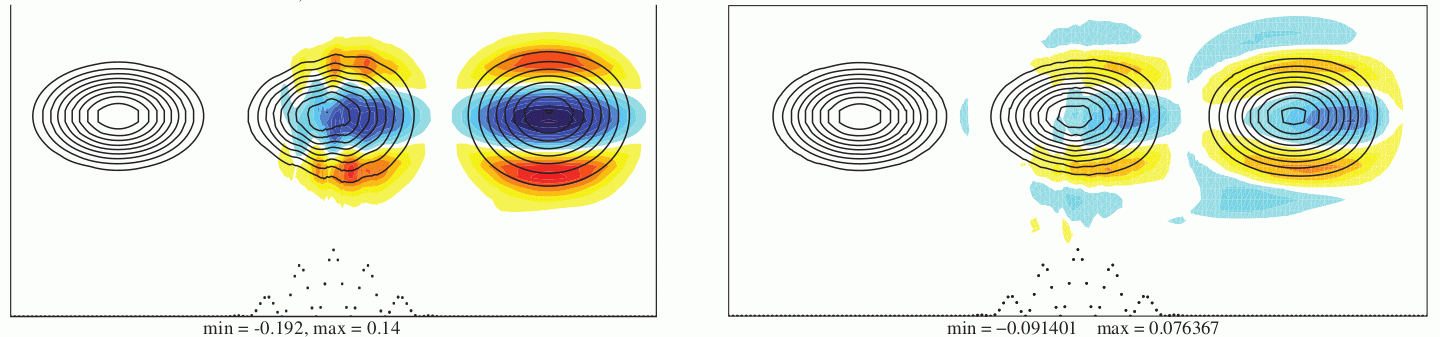
\includegraphics[width=\linewidth]{ChenFig7.png}
\caption{From figure 7 of \cite{CWPS17} with contours showing concentration of a tracer at three times begin advected over a mountain range on a highly distorted, terrain following grid. A dimensionally split, COSMIC scheme without a limiter is used for the left hand results and a second-order multi-dimensional scheme for unstructured grids is used for the results on the right. Colours and the max and min values show errors.}
\label{fig:CWPS17_fig7}
\end{figure}

\todo[inline]{James, please feel free to replace this with some of your work. This is just a place holder. You can probably do something better.}

\end{itemize}

\subsubsection*{Responses to Reviewer 167069074}

We are pleased that the reviewer thought that our work will deliver ``important contributions'', that our expertise is ideal and that the reviewer appreciated the ``strong support from the Met Office and ECMWF''. 

\begin{enumerate}
\item While the reviewer found the proposal ``strong on the strategy and approach'' they asked about how we plan to evaluate the schemes. PI Kent is a world expert on evaluating transport schemes \cite[]{KENT2014b,KENT2014c,KENT2012a,KENTHOLDAWAY,KENT2014a,DCMIP2016}, developing test cases that have been widely used and providing evaluations that have impacted operational models. For the proposed work, we have a number of evaluation plans:
    \begin{enumerate}
    \item We will use existing test cases where possible and rank schemes in terms of error, conservation, boundedness, correlation preservation and efficiency metrics. 
    \item The parallel efficiency will be evaluated using profiling tools, as described in WP1 under PI Maynard's supervision.
    \item WP2 proposes that a ``new set of idealised test cases will be developed using re-analysis winds''. For these we will calculate error metrics in comparison to a high resolution reference solution and assess how accuracy and stability varies with time step.
    \item As described in WP3, we will use some of the same evaluation methods as ECMWF.
    \item Limited test cases exist to evaluate non-linear advection schemes, as described in TC4. More work will be needed to find suitable evaluation of a three dimensional solver for Burger's equation which we feel that we are well placed to deliver this.
    \item For the multi-fluid modelling the focus is on finding schemes that are stable and accurate for long time steps. Therefore we will compare simulations with long and short time steps. This evaluation is particularly straightforward as it is simple to calculate error metrics between simulations with the same spatial resolution. 
    \end{enumerate}

\item In contrast to the other reviewers, the reviewer was concerned that the contributions from the Met Office and ECMWF were insufficient. 
This work is not a sub-contract from operational centres. We are exploring new, innovative approaches that could be too risky for an operational centre to commit significant resource to. Due to the importance of the work, both ECMWF and the Met Office have their own plans for developing a suitable advection scheme -- they are not completely reliant on this project. We will be involved in their plans -- comparing results and discussing new ideas, but we are not part of their teams, we are independent and will pursue our own ideas and we will take greater risks, spending more time on innovative approaches. We do not believe that we need to do more in our impact work -- if we find a better advection scheme that fits within the Met Office or ECMWF frameworks, it is very likely to be adopted due to the frequent communication between us and the importance of of the topic.

\item Respond to \todo[inline]{I was less than clear about the roles of the USW staff in the work flow. There is no real description of this. The PDRA will work for the first 24 months so presumably only contributes to WP1 and WP2. Is the PI's 30\% to cover the work in WP4?
What is the role of the student mentioned, are they central to the WPs or add further value to the work programme? There
is no real detail on this at all.}

\item Respose to \todo[inline]{I find the 7 overseas conferences for a 3 year standard grant very excessive. It seems very difficult to me to justify this but
no attempt is made to do so in the proposal.
The 30\% PI time is not justified at all in my view. There is no real breakdown of the staff roles and activities in the case for
support or the JoR.}

The reviewer was concerned that we are planning to attend too many international conferences. We would like this work to have impact beyond the Met Office and ECMWF and this work will have impact if the results are communicated to operational centres and other model developers. We will choose to attend international conferences attended by operational centres. It is also important for the PDRAs to attend conferences for their continued professional development and future career opportunities. So we think that one international conference per PDRA per year and one international conference for Kent and one for Weller is suitable. 

We answer the point about the 30\% PI time at USW above.

We welcome the opportunity to say more about the staff roles at Reading. PI Maynard will contribute to WP1, undertaking the work on parallel performance and profiling. WP3 will be carried out at Reading, with PI Weller supervising the Reading PDRA. Part 3 of WP4 (solving Burger's equation) will be led by PI Weller in Reading. WP5 will be carried out at Reading, led by PI Weller.

\end{enumerate}

\subsubsection*{Responses to Reviewer 171942111}

We appreciate that the reviewer has confidence in our expertise to deliver on this timely project, pleased that they consider our links with the Met Office and ECMWF excellent and pleased they they find our impact plan appropriate.

We respond to the point about the split between the USW PI and PDRA above.

We appreciate the reviewers confidence in our plan to compare a range of methods. The reviewer rightly questions how we plan to generalise the accurate efficient transport on structured grids to arbitrary grids. We have three potential approaches described in WP3. The first two, revisiting implicit time-stepping and local sub-stepping are not a mystery. The third -- generalising FFSL to arbitrary grids is a way in which the cost does not scale with Courant number is more uncertain. ...

%\begin{multicols}{2}
\renewcommand{\refname}{References}
\bibliography{Weller,Kent,Maynard}
\bibliographystyle{abbrvnat2}
%\end{multicols}

\end{document}
